% !TEX TS-program = pdflatex
% !TEX encoding = UTF-8 Unicode

% This is a simple template for a LaTeX document using the "article" class.
% See "book", "report", "letter" for other types of document.

\documentclass[11pt]{article} % use larger type; default would be 10pt

\usepackage[utf8]{inputenc} % set input encoding (not needed with XeLaTeX)

%%% Examples of Article customizations
% These packages are optional, depending whether you want the features they provide.
% See the LaTeX Companion or other references for full information.

%%% PAGE DIMENSIONS
\usepackage{geometry} % to change the page dimensions
\geometry{a4paper} % or letterpaper (US) or a5paper or....
% \geometry{margin=2in} % for example, change the margins to 2 inches all round
% \geometry{landscape} % set up the page for landscape
%   read geometry.pdf for detailed page layout information

\usepackage{graphicx} % support the \includegraphics command and options

% \usepackage[parfill]{parskip} % Activate to begin paragraphs with an empty line rather than an indent

\usepackage{amsmath} %math

%%% PACKAGES
\usepackage{booktabs} % for much better looking tables
\usepackage{array} % for better arrays (eg matrices) in maths
\usepackage{paralist} % very flexible & customisable lists (eg. enumerate/itemize, etc.)
\usepackage{verbatim} % adds environment for commenting out blocks of text & for better verbatim
\usepackage{subfig} % make it possible to include more than one captioned figure/table in a single float
% These packages are all incorporated in the memoir class to one degree or another...

%%% HEADERS & FOOTERS
\usepackage{fancyhdr} % This should be set AFTER setting up the page geometry
\pagestyle{fancy} % options: empty , plain , fancy
\renewcommand{\headrulewidth}{0pt} % customise the layout...
\lhead{}\chead{}\rhead{}
\lfoot{}\cfoot{\thepage}\rfoot{}

%%% SECTION TITLE APPEARANCE
%\usepackage{sectsty}
%\allsectionsfont{\sffamily\mdseries\upshape} % (See the fntguide.pdf for font help)
% (This matches ConTeXt defaults)

%%% ToC (table of contents) APPEARANCE
\usepackage[nottoc,notlof,notlot]{tocbibind} % Put the bibliography in the ToC
\usepackage[titles,subfigure]{tocloft} % Alter the style of the Table of Contents
\renewcommand{\cftsecfont}{\rmfamily\mdseries\upshape}
\renewcommand{\cftsecpagefont}{\rmfamily\mdseries\upshape} % No bold!

%%% END Article customizations

%%% The "real" document content comes below...

\title{Tetris with Gravity}
\author{Nordberg, Marcus \\ mnordber@kth.se
		\and
	Rolleberg, Niklas \\ nrol@kth.se}
%\date{} % Activate to display a given date or no date (if empty),
         % otherwise the current date is printed 

\begin{document}
\maketitle
\tableofcontents
\newpage
\section{Project idea}
Our idea for a project was to make a version of Tetris with physical forces and behaviour of the Tetris blocks. The goal of the project was to make Tetris look more realistic. 

\section{Restrictions}
Due to the short timespan we had to make some restrictions to the game. We decided to use spheres instead of squares, so that collision detections would be easier, and we would not have to consider rotations from collisions.

\section{Technical aspects}
Forces needed for this project is a gravitational force, a force keeping the Tetris blocks together and some sort of wall collision force.

The forces implemented in this project are all spring-based, except for the gravity. First we tried to make the spheres bounce on the walls and eachother just by handling these collisions as fully elastic collisions. This, however, did not look very realistic. Instead we decided to give up the collision-approach and go for a mass-spring system instead. In order for this to work we had to implement Hooke's law \eqref{eq:hookeslaw} and a damper to prevent oscillations \eqref{eq:damping}.
%Hooke's law
\begin{equation}
	\label{eq:hookeslaw}
       F = -k*X
\end{equation}

where $k$ is the spring constant and $X$ is the difference in length compared to the relaxed length of the spring.

\begin{equation}
	\label{eq:damping}
       F = -d*V
\end{equation}

where $d$ is the damping factor and $V$ is the velocity of the sphere.

Whenever a sphere would collide with the wall or ground, a spring is introduced. This spring will have the ``relaxed length'' of $1 * r$ where $r$ is the radius of the sphere. The result of this is a force directed from the wall.

The same logic applies whenever two spheres collides. Detecting collision between two spheres is simple ($if~d < 2 * r$) and resolving the collision comes down to introducing a spring between the two center-points. This spring has a ``relaxed length'' of $2 * r$ and thus, will force the spheres to disperse.

In both of these cases, we had to tweak the numbers (spring constant and damping) quite a lot to get realistic results.
\section{Game aspects}
Implementing physics and getting the model to work was the priority of this project. Adding game mechanics and making it enjoyable to play was a stretch goal. We found that it is quite hard to build upon a physics simulation and try to build the game mechanics around that.

What makes Tetris hard is that you are often getting into situation where your new Tetris blocks does not really fit anywhere. This is not the case in our rendition of Tetris as physics makes the block kind of fall into places.

We had to think outside the box and come up with a new way to play Tetris. An early idea was to make all spheres without a connection disappear. As Tetris blocks break into spheres when a large enough force is applied, this would mean that the game would be about demolision. This did not feel quite right as it felt too far from original Tetris and there was not really any benefit from not moving at all and just drop the blocks. We had to go back to the drawing board. The next idea was to add requirements for the full rows. Instead of just accepting any full row, we could require that at least five colors were represented in this row and have the Tetris blocks in different colors. This felt more like Tetris and actually made the game quite hard. 

\section{Implementation}
In our first attempt, we tried to use fully elastic collisions. We succeeded with getting fairly realistic interaction between the ground and a bouncing ball, but as we added more spheres, things started to go south. The interaction between spheres was not realistic at all, mostly because we had to cancel out chain reactions between the spheres with a high dampening. This made the spheres move slowly colliding, which didn't look realistic at all.

Our implementation of the mass spring system is based on lab 3. We started out by using the euler method for calculating the movement of the spheres, this turned out to be a problem because of the low accuracy and small stability region of the method. When the spheres were supposed to be stationary they ware bouncing up and down slightly instead. We tried to counteract this by increasing the spring coefficient but this made the system unstable, and the spheres started flying in all directions. To solve this we changed numerical integrator to RK4 which is a method with a fourth order accuracy compared to to forward euler which is just first order. RK4:s stability region is also bigger than forward euler which allowed us to have larger forces while maintaining the same time step.

While there is a larger risk of performance issues when using RK4, Tetris is very limited in terms of amount of processing. We know the possible maximum of objects on the screen during a game so as long as we can handle that scenario, performance will not be an issue.

Moving on, we would like to implement some sort of space partitioning for the collision detection. It doesn't make sense to check for all collisions at all time. As the game is already row partitioned (The board is divided into rows and each sphere belongs to the row of which it has its center point in.) we think that it would be pretty easy to also implement some sort of column partitioning to further improve performance. While the performance is not a problem right now, it could become a problem if we were to introduce textures or more advanced graphical effects.

\subsection{Our Work Flow}
We think that our work flow was really good for this project. The milestones we set up were realistic and we managed to held all our internal deadlines. Our first milestone was to get a single sphere to bounce. This meant that we had to solve collision between borders and the spheres. Extending from this, the next milestone was to add additional spheres for sphere-to-sphere collision. The last milestone was to build a Tetris block consisting of small spheres and make it work. We feel like this was a good way of conducting this project. When we found time before the deadline, we focused on game mechanics and enjoyability.

\subsection{How we divided the work}
We did most of the project work together. Marcus did the most of the coding, and Niklas did most of the work related to the physics model. 

\subsection{Final results}
\begin{center}
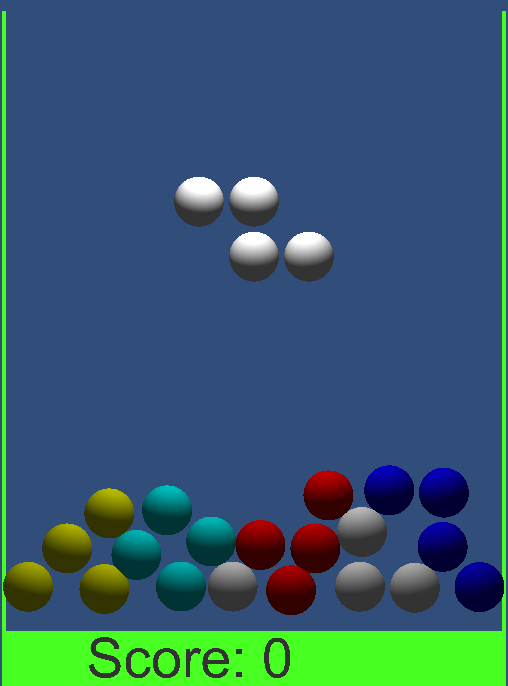
\includegraphics[scale=0.3]{bild1.png}
\end{center}


\section{Conclusion}
Simulations are all about selling something fake to an audience. In the end, a simulation's purpose is to trick someone into believing something. During the work in progress seminar, one of the TA's said that they actually liked one of the first versions of Jonathan's bowling ball\footnote{http://jonathangolan.se/Blog/blog.html}. The TA had a different opinion (or idea) of what a bowling ball hitting a brick wall would look like. Sadly, we never hit this road block which, according to us, is one of the most interesting parts about models and simulation. When you have to take a step back and think for a second -- what is really the most realistic simulation of this problem? According to whom?

There are still things in our project that we would not be able to sell to an audience. The way spheres slowly drifts outside the borders and the way they might intersect is simply not realistic. 

\section{Ideas for further work}
\begin{itemize}
\item{Add friction so the spheres behave less like a liquid -- This is important for the walls as all the spring forces makes the spheres closest to the walls slowly climb them.}
\item{Change the spheres to squares, and consider rotation -- A huge amount of our code is based around spheres so changing to cubes would mean a lot of work but the result could be really good. It would be easier to identify it as Tetris.}
\item{Add spheres with different attributes, like mass, other forces, etc. -- This would add to the game mechanics and enjoyability}
\item{Extend to 3D -- While easy to do it would add extra challenges on the game mechanics. How would a 3D version of Tetris work?}
\item{Add more interesting game mechanics}
\end{itemize}

\end{document}
